\section{Rappels : concepts et outils fondamentaux de l'aléatoire}\label{concepts}

\begin{remark}
Pour faciliter la lecture et l'appropriation, cette annexe de rappels est illustrée par de nombreux exemples de phénomènes naturels dits \emph{extrêmes}, telles des pluies diluviennes, des vents forts, etc. dont on cherche à modéliser le comportement. 
\end{remark}


La mod\'elisation probabiliste d'un al\'ea $X$ repose sur le caract\`ere de {\it variable al\'eatoire} conf\'er\'e \`a $X$, \'evoluant dans un ensemble d'\'echantillonnage $\Omega$ de dimension $d$. Puisque $\Omega\neq\varnothing$, les sous-ensembles de valeurs ${\cal{A}}\subset\Omega$ que peut parcourir $X$ sont non vides, et ils pr\'esentent une certaine stabilit\'e : l'union d\'enombrables de plusieurs ${\cal{A}}_i$ est encore dans $\Omega$, de m\^eme que le compl\'ementaire de tout sous-ensemble ${\cal{A}}$. \\

 Ces propri\'et\'es fondamentales permettent de ``paver" ({\it mesurer}) l'ensemble $\Omega$ de fa\c con \`a associer \`a toute observation (survenue) d'un {\it \'ev\'enement} $A\in{\cal{A}}$ %\footnote{Le terme d'{\it \'ev\'enement} renvoie, dans ce paragraphe, uniquement \`a la d\'efinition usuelle des \'el\'ements d'une tribu ou $\sigma-$alg\`ebre ${\cal{A}}$ et non aux ``\'ev\'enements" naturels qui sont \'evoqu\'es en continu dans ce cours. } 
  une valeur num\'erique $\Pm(A)$. L'ensemble de ces valeurs num\'eriques vit dans l'intervalle $[0,1]$, et est tel que 
$$
\Pm(\Omega) = 1.
$$ 
On parle alors, pour d\'esigner $\Pm$, de {\it mesure de probabilit\'e}. \\ 

La th\'eorie des probabilit\'es nomme  le triplet $(\Omega,{\cal{A}},\Pm)$  {\it espace probabilis\'e}, l'ensemble $\Omega$ {\it univers} et ${\cal{A}}$  {\it tribu} (ou $\sigma-$alg\`ebre). En g\'en\'eral, le choix de ${\cal{A}}$ est l'ensemble des parties de $\Omega$ dont la mesure de Lebesgue peut \^etre d\'efinie (cf. $\S$ \ref{unidim.chap1}). %, la {\it tribu de Lebesgue}. 
Il n'est donc usuellement pas donn\'e de pr\'ecision, dans les probl\`emes appliqu\'es, sur ${\cal{A}}$. \\



%%%%%%%%%%%%%%%%%%%%%%%%%%%%%%%%%%%%%%%%%%%%%%%
\subsection{Probl\`emes unidimensionnels}\label{unidim.chap1}

Consid\'erons tout d'abord le cas o\`u $d=1$. Si $\Omega$ est {\it discret} (par exemple si $\Omega=\{1,2,3,\ldots,\}$) ou {\it cat\'egoriel}, et plus g\'en\'eralement si $\Omega$ est {\it d\'enombrable}, la distribution de probabilit\'e est dite discr\`ete et est d\'etermin\'ee par la {\it fonction de masse} probabiliste 
$$
f(x) = \Pm(X=x)
$$
pour toute valeur $x\in\Omega$. Cependant, la tr\`es grande majorit\'e des variables al\'eatoires consid\'er\'ees dans ce cours pr\'esente un caract\`ere {\it continu}. En particulier, les valeurs prises par $X$ (vitesse du vent, temp\'erature, d\'ebit d'une rivi\`ere...) \'evoluent contin\^ument -- ce qui est indispensable pour appliquer la th\'eorie des valeurs extr\^emes -- et $\Omega$ constitue g\'en\'eralement un sous-ensemble continu de $\R^d$, m\^eme si le dispositif de mesure est n\'ecessairement limit\'e, en pratique, par une pr\'ecision donn\'ee. Cette pr\'ecision ne joue pas de r\^ole dans la construction du mod\`ele probabiliste mais dans celui du mod\`ele {\it statistique}, qui englobe le mod\`ele probabiliste en \'etablissant un lien direct avec des observations bruit\'ees (voir $\S$ \ref{confusion.modele}). Dans la pratique, les deux  mod\`eles sont  confondus quand le bruit d'observation est consid\'er\'e comme n\'egligeable. \\

Dans le cas continu, c'est-\`a-dire lorsque $\Omega$ n'est plus d\'enombrable, la distribution de probabilit\'e peut \^etre sp\'ecifi\'ee par la {\it fonction de r\'epartition} \index{{fonction de r\'epartition}@{fonction de r\'epartition}}
$$
F_X(x) = \Pm(X\leq x)
$$
pour toute valeur $x\in\Omega$. Afin de satisfaire les axiomes des probabilit\'es \cite{kolmogorov1950}, cette fonction doit \^etre croissante, et telle que, lorsque la dimension $d=1$, 
\begin{eqnarray*}
\lim\limits_{x \to x_{\inf}} F_X(x) & = & 0, \\
\lim\limits_{x \to x_{\sup}} F_X(x) & = & 1 \\
\end{eqnarray*}
o\`u $(x_{\inf},x_{\sup})$ sont les bornes inf\'erieure et sup\'erieure (\'eventuellement infinies) de $\Omega$. Le cas multidimensionnel o\`u $d>1$ est pr\'ecis\'e au $\S$ \ref{axiomes.multidim}. Toujours pour $d=1$, l'\'equivalent de la probabilit\'e  discr\`ete $f(x)$ dans le cas continu est fourni par la probabilit\'e que $X$ se situe entre les valeurs $x-a$ et $x+b$ (avec $a,b\geq 0$) :
$$
\Pm(x-a \leq X \leq x+b) = F_X(x+b) - F_X(x-a).
$$
Cette propri\'et\'e pousse \`a d\'efinir, dans les cas o\`u $F_X$ est d\'erivable, la d\'eriv\'ee de $F_X$ (dite {\it de Radon-Nikodym-Lebesgue}) d\'efinie comme le cas-limite $a=b=\epsilon\to 0$  
$$
f_X(x) = \frac{d F_X}{d x}(x),
$$
appel\'ee {\it densit\'e de probabilit\'e} de $X$, \index{{densit\'e}@{densit\'e}} qui est donc telle que
$$
F(x) = \int_{-\infty}^x f_X(u) \ du
$$      
et
$$
\Pm(x-a \leq X \leq x+b) = \int_{x-a}^{x+b} f_X(u) \ du. 
$$
N\'ecessairement, $\int_{\Omega} f_X(u) \ du =1$. 
Ainsi, toute distribution de probabilit\'e continue, en dimension $d=1$ (c'est aussi le cas en dimension $d>1$) peut \^etre repr\'esent\'ee de fa\c con \'equivalente (sous r\'eserve de d\'erivabilit\'e\footnote{Plus g\'en\'eralement de {\it diff\'erentiabilit\'e} en dimension quelconque.}) par sa fonction de r\'epartition ou sa densit\'e (figure \ref{chapitre1-fig1a}). \\

Informellement, $f_X$ peut \^etre vue comme la limite de l'histogramme en fr\'equence des valeurs possibles de $X$, pour des classes de valeurs \'etroites (figure \ref{chapitre1-fig1a}). Plus formellement, fonction de r\'epartition et densit\'e de probabilit\'e doivent \^etre interpr\'et\'ees comme des outils permettant d'op\'erer une {\it mesure} \index{{mesure}@{mesure}} de la distribution des $X$ relativement \`a une mesure de l'espace $\Omega$. \\



\begin{figure}[h!] %btp]
 % \vspace{5.5cm}
	\centering
	\hspace{-1.5cm}
	\begin{minipage}[c]{.46\linewidth}
      %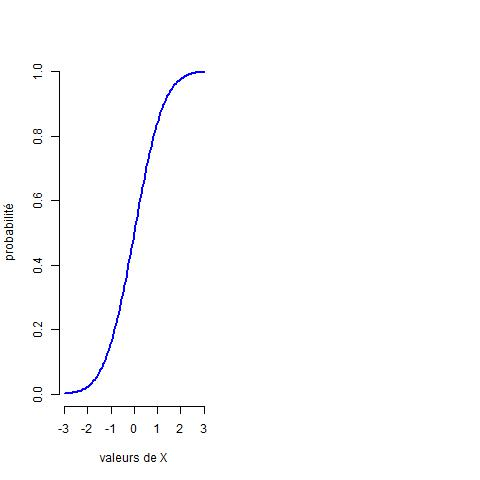
\includegraphics[scale=0.65,natwidth=5cm,natheight=3cm]{figures/concepts/chapitre1-fig1-1.jpeg}
       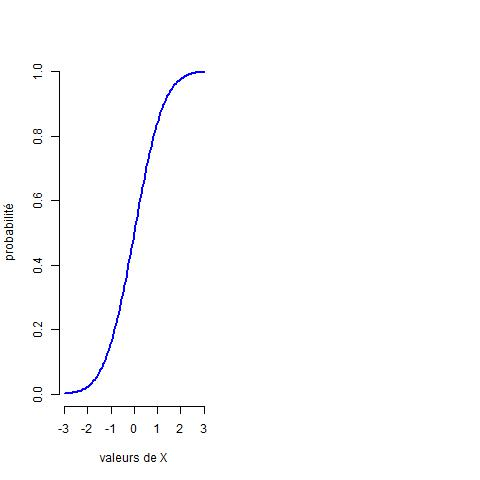
\includegraphics[scale=0.4]{figures/concepts/chapitre1-fig1-1.jpeg}
			%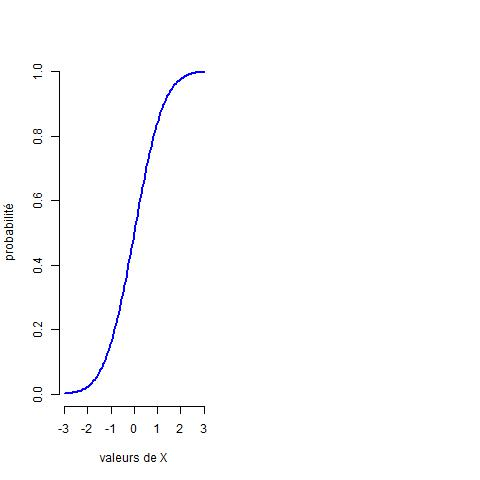
\includegraphics[width=6cm,height=6cm,natwidth=5cm,natheight=3cm]{figures/concepts/chapitre1-fig1-1.jpeg}
			\end{minipage} \hspace{-0.75cm}
   \begin{minipage}[c]{.46\linewidth}
	%\hspace{-0.5cm}
			%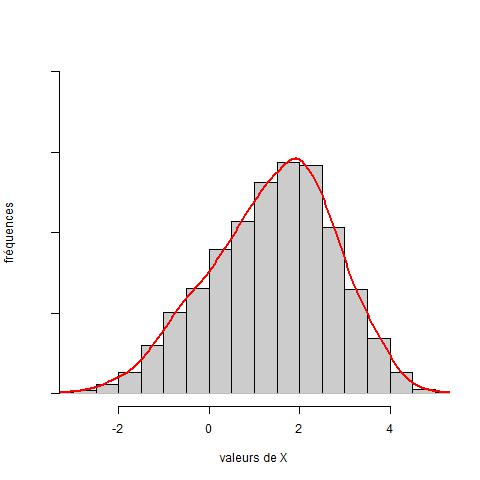
\includegraphics[scale=0.65,natwidth=4cm,natheight=4cm]{figures/concepts/chapitre1-fig1-2.jpeg}
			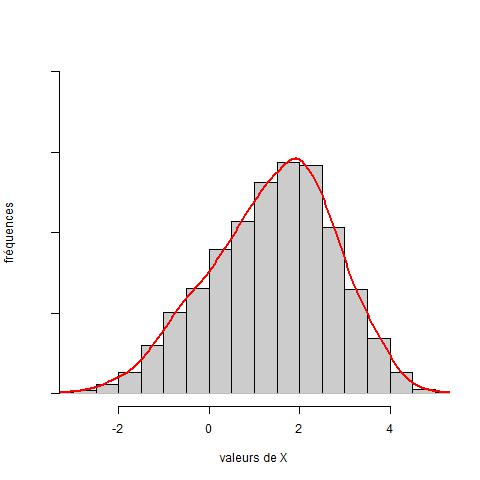
\includegraphics[scale=0.4]{figures/concepts/chapitre1-fig1-2.jpeg}
			%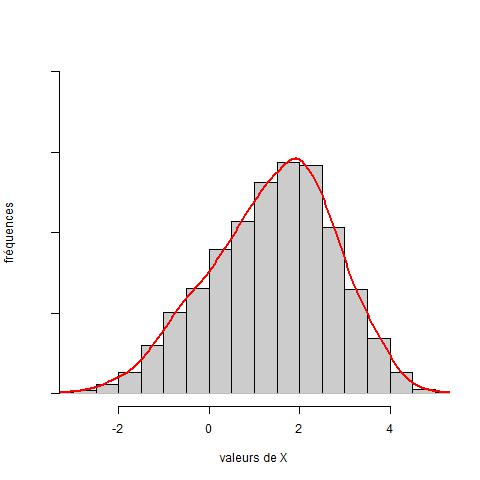
\includegraphics[width=6cm,height=6cm,natwidth=4cm,natheight=4cm]{figures/concepts/chapitre1-fig1-2.jpeg}
			\end{minipage}
	\caption{
      \label{chapitre1-fig1}
   Gauche : exemple de fonction de r\'epartition. Droite : histogramme en fr\'equence de valeurs de $X$ et densit\'e de probabilit\'e correspondante (courbe).}
  %\end{center}
\end{figure}

Consid\'erons par exemple que $\Omega=I_1\times I_2\times \ldots \times I_d$, o\`u chaque $I_k$ est un intervalle de $\R$ (ferm\'e, ouvert ou semi-ouvert), l'ensemble constituant un parall\'el\'epip\`ede contenant toutes les valeurs de $X$ pouvant \^etre observ\'ees. Ce solide (ou cet espace) peut \^etre d\'ecrit par un ensemble de mesures, par exemple son volume. La mesure de Lebesgue \cite{lebesgue1972}, not\'ee $\mu_L$,  \index{{mesure de Lebesgue}@{mesure de Lebesgue}} a \'et\'e construite comme une mesure de r\'ef\'erence permettant de d\'ecrire ce type d'espace de fa\c con universelle et uniforme. Comme le volume, elle prend une valeur finie si $\Omega$ est compact. La densit\'e $f_X$ d\'efinit une autre mesure sur $\Omega$, qui sp\'ecifie la forme de la distribution des $X$ et permet de la diff\'erencier de l'uniformit\'e. Il faut donc l'interpr\'eter comme une mesure {\it relative} \`a celle de Lebesgue (ou {\it domin\'ee} par la mesure de Lebesgue). Au  lecteur int\'eress\'e par une introduction d\'etaill\'ee \`a la th\'eorie de la mesure, nous sugg\'erons les ouvrages \cite{Bouleau1986} (pour une approche "ing\'enieure") et \cite{LeGall2006} (pour une vision plus math\'ematique). \\

L'information incertaine transport\'ee par les distributions de probabilit\'e est tr\`es souvent r\'esum\'ee par des indicateurs statistiques particuliers : les {\it moments} d'ordre $k\in\N$, d\'efinis comme l'ensemble des valeurs moyennes de la variable $X^k$ : \index{{moment}@{moment}}
$$
M_k = \E[X^k] = \int_{\Omega} x^k f_X(x) \ dx.
$$
Si ceux-ci existent pour $k=1$ et $k=2$, ils permettent de d\'efinir l'{\it esp\'erance} $\E[X]$ \index{{esp\'erance}@{esp\'erance}} et la {\it variance} \index{{variance}@{variance}}
\begin{eqnarray*}
\V[X] & = & \int_{\Omega} \left(x-\E[X]\right)^2 f_X(x) \ dx.
\end{eqnarray*}
L'esp\'erance fournit une mesure de localisation moyenne de $X$ dans la distribution $f_X$, tandis que $\V[X]$ est une mesure de la variabilit\'e (ou dispersion) de $f_X$. L'{\it \'ecart-type} de $f_X$, homog\`ene \`a $X$, est d\'efini par 
$$
\sigma_X=\sqrt{\V[X}].
$$ 
Alternativement, le {\it c{\oe}fficient de variation} de $X$ \index{{c{\oe}fficient de variation}@{c{\oe}fficient de variation}}
$$
\CV[X] = \frac{\sigma_X}{\E[X]},
$$
fournit une autre mesure {\it relative} de la variabilit\'e ou dispersion de $f_X$ (plus usuelle pour les ing\'enieurs). Enfin, on parlera de variable centr\'ee-r\'eduite si $X$ est transform\'ee en \index{{variable centr\'ee r\'eduite}@{variable centr\'ee r\'eduite}}
$$
X' = \frac{X-\E[X]}{\sigma_X},
$$
d'esp\'erance nulle et de variance unitaire. 

\subsection{Familles de mod\`eles param\'etriques}\label{lois}

Rappelons quelques mod\`eles probabilistes ou statistiques fondamentaux, qui interviennent tr\`es souvent dans les constructions plus \'elabor\'ees qui seront d\'ecrites dans ce cours. Ces mod\`eles seront, dans le cadre de ce cours, consid\'er\'es {\it param\'etriques}, c'est-\`a-dire descriptibles de fa\c con exhaustive par un ensemble fini de param\`etres. \index{{mod\`ele param\'etrique}@{mod\`ele param\'etrique}} \\

La premi\`ere raison de ce choix est li\'ee au cadre d'\'etude : le comportement des extr\^emes d'un \'echantillon al\'eatoire suit, sous certaines conditions th\'eoriques, des lois param\'etriques. C'est aussi le cas du comportement des estimateurs statistiques ($\S$ \ref{estimation.stat.classique}) ob\'eissant \`a une loi des grands nombres. 

Cet argument fondamental se renforce de la constatation suivante : lorsqu'on s'int\'eresse \`a ces comportements extr\^emes, le nombre d'observations disponibles devient faible. Expliquer la production de ces observations par un m\'ecanisme al\'eatoire d\'etermin\'e par un nombre infini %(de fa\c con {\it non-param\'etrique}) 
ou m\^eme simplement grand de param\`etres (c'est-\`a-dire plus grand que le nombre de donn\'ees) semble d\'eraisonnable car la majeure partie de ces param\`etres resteront inconnus, ou poss\`ederont plusieurs valeurs possibles, et le mod\`ele ainsi cr\'e\'e ne serait pas identifiable et utilisable. \\

Dans ce document, on notera tr\`es g\'en\'eralement $\theta$ ce vecteur de param\`etres, qui \'evoluera donc dans un espace $\theta$ de dimension finie. Le conditionnement \`a $\theta$ du m\'ecanisme de production al\'eatoire sera rappel\'e dans les notations des densit\'es et fonctions de r\'epartition : $f_X(x)=f(x|\theta)$ et $F_X(x)=F(x|\theta)$.

\subsubsection*{Lois}\label{lois.para}

Dans un cadre discret, on peut s'int\'eresser \`a la survenue d'un \'ev\'enement ponctuel $Z>z_0$, o\`u $Z$ est, par exemple, un niveau d'eau maximal mensuel, et $z_0$ une hauteur de digue de protection. Supposons disposer d'un \'echantillon d'indicateurs $(\delta_1,\ldots,\delta_n)\in\{0,1\}^n$ valant chacun 1 si la crue ainsi d\'efinie survient, et 0 sinon.  Faisons l'hypoth\`ese que les $\delta_i$ sont ind\'ependants et correspondent chacun au r\'esultat d'un ``essai de submersion" r\'eussissant avec une m\^eme probabilit\'e $p$. Si l'on note $X_n=\sum_{i=1}^n \delta_i$ le nombre total de ``succ\`es" parmi ces $n$ essais, alors la fonction de masse probabiliste de $X_n$ s'\'ecrit
$$
f(x) = \left(\begin{array}{l} n \\ x \end{array}\right) p^x (1-p)^{n-x}
$$
pour $x\in\Omega=\{0,1,2,\ldots,n\}$, et o\`u
$$
\left(\begin{array}{l} n \\ x \end{array}\right) = \frac{n!}{x!(n-x)!}.
$$
La variable al\'eatoire $X_n$ est alors dite suivre la {\it loi binomiale} \index{{loi binomiale}@{loi binomiale}} ${\cal{B}}(n,p)$ (figure \ref{chapitre1-fig1a}). Dans le cadre d'une \'etude de risque, on s'attachera \`a  estimer la probabilit\'e de surverse $p$ \`a partir de la statistique observ\'ee $x_n$. \\

La variable  $X_n$ dite de {\it comptage} d\'efinie ci-dessus peut \^etre g\'en\'eralis\'ee dans une perspective d'estimer l'occurence d'\'ev\'enements survenant de fa\c con al\'eatoire durant un laps de temps fix\'e (par exemple une ann\'ee). Si on suppose que ces \'ev\'enements surviennent avec une fr\'equence moyenne unique $\lambda>0$ dans cet intervalle de temps, alors la probabilit\'e qu'il survienne exactement $X_n=x\in\Omega=\{0,1,\ldots,\infty\}$ occurences est
$$
f(x) = \frac{\lambda^x}{x!} \exp(-\lambda),
$$  
qui d\'efinit la fonction de masse probabiliste de la {\it loi de Poisson} \index{{loi de Poisson}@{loi de Poisson}} d'esp\'erance $\lambda$ (figure \ref{chapitre1-fig1a}). Celle-ci joue notamment un grand r\^ole dans l'\'etablissement des lois  statistiques associ\'ees aux observations historiques car elle permet de mod\'eliser la survenue du nombre d'\'ev\'enements situ\'es entre deux dates (par exemple s\'epar\'es par plusieurs dizaines d'ann\'ees) et non observ\'es directement. Le lien technique entre la loi binomiale et la loi de Poisson s'exprime dans le lemme suivant : \\

\begin{lemmo}
Si $X_n$ suit une loi binomiale ${\cal{B}}(n,p)$ avec $p\ll 1$, alors la loi de $X_n$ peut \^etre approxim\'ee par la loi de Poisson d'esp\'erance $np$ lorsque $n\to\infty$. \\
\end{lemmo}


Rappelons enfin, dans le cas continu, l'importance fondamentale de la {\it loi normale} $X\sim {\cal{N}}(\mu,\sigma^2)$, \index{{loi normale}@{loi normale}} d'esp\'erance $\mu$ et de variance $\sigma^2$, et de densit\'e de probabilit\'e (pour $d=1$ et $\Omega=\R$) 
\begin{eqnarray*}
f_X(x) & = & \frac{1}{\sqrt{2\pi}\sigma} \exp\left(-\frac{1}{2\sigma^2}(x-\mu)^2 \right).
\end{eqnarray*}
Celle-ci mod\'elise un grand nombre de ph\'enom\`enes, en particulier celui de la r\'epartition de la moyenne d'un \'echantillon al\'eatoire (loi des grands nombres).   La convergence en loi  normale d'un estimateur statistique (cf. $\S$ \ref{convergence}) constitue un type de r\'esultat tr\`es classique (th\'eor\`eme de la limite centrale). 
La variable $(X-\mu)/\sigma$ suit la loi normale dite {\it centr\'ee r\'eduite} ${\cal{N}}(0,1)$ (figure \ref{chapitre1-fig1a}). On note usuellement par $\phi(.)$ et $\Phi(.)$ les densit\'e et fonction de r\'epartition de cette loi centr\'ee r\'eduite. \\


\begin{figure}[h!] %btp]
  %\vspace{5.5cm}
	\centering
	\hspace{-2cm}
	\begin{minipage}[c]{.46\linewidth}
      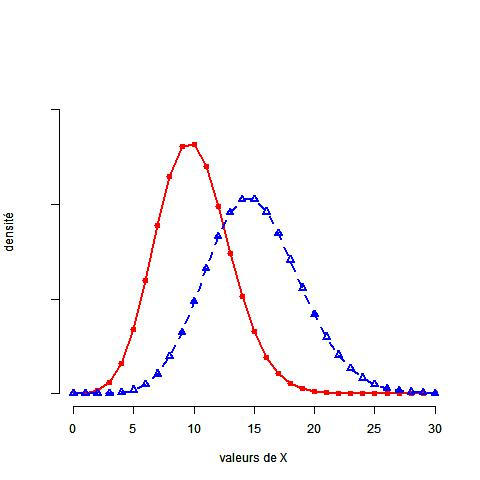
\includegraphics[scale=0.5]{figures/concepts/chapitre1-fig2-1.jpeg}
			\end{minipage} %\hfill \
			%\hspace{-0.4cm}
   \begin{minipage}[c]{.46\linewidth}
	%\hspace{-0.5cm}
			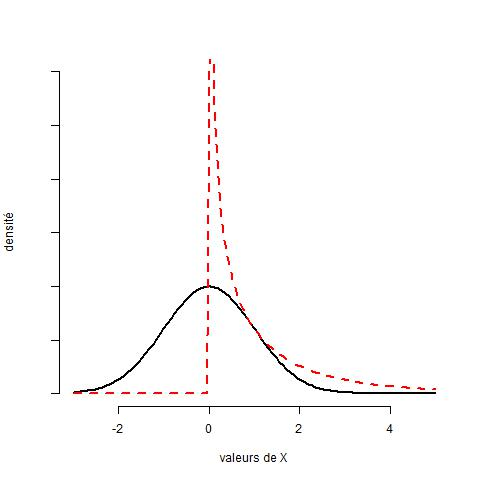
\includegraphics[scale=0.5]{figures/concepts/chapitre1-fig2-2.jpeg}
			\end{minipage}
	\caption{
      \label{chapitre1-fig1a}
      Gauche : fonction de masse des lois discr\`etes binomiale ${\cal{B}}_n(100,0.1)$ (carr\'es) et Poisson ${\cal{P}}(15)$ (triangles). Droite : densit\'es de probabilit\'e continues de la loi normale centr\'ee r\'eduite ${\cal{N}}(0,1)$ (courbe pleine) et $\chi^2_1$.}
\end{figure}

%\begin{figure}[hbtp]
  %\begin{center}
       %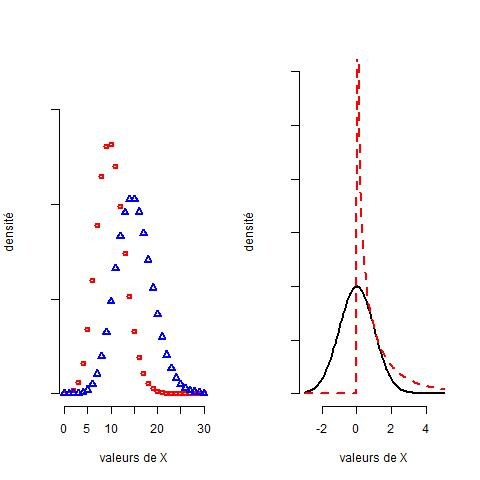
\includegraphics[scale=0.7,natwidth=620,natheight=420]{figures/concepts/chapitre1-fig2.jpeg}
	%\caption{
      %\label{chapitre1-fig2}
   %Gauche : fonction de masse des lois discr\`etes binomiale ${\cal{B}}_n(100,0.1)$ (cercles) et Poisson ${\cal{P}}(15)$ (triangles). Droite : densit\'es de probabilit\'e continues de la loi normale centr\'ee r\'eduite ${\cal{N}}(0,1)$ (courbe pleine) et $\chi^2_1$.}
  %\end{center}
%\end{figure}

\subsubsection*{Tests statistiques}\label{test.statistique.classique}

La d\'emarche g\'en\'erale des tests consiste \`a rejeter ou ne pas rejeter (sans forc\'ement accepter) une hypoth\`ese statistique $H_0$, dite {\it nulle}, en fonction d'un jeu de donn\'ees ${\bf x_n}$. Par exemple, dans un cadre param\'etrique cette hypoth\`ese peut correspondre au  choix sp\'ecifique d'une valeur $\theta=\theta_0$ dans une m\^eme famille $f(x|\theta)$ ou d'un domaine $\theta\in\theta_0$. D\'efinir un test revient \`a d\'efinir une statistique
\begin{eqnarray*}
R_n & = & R(X_1,\ldots,X_n)
\end{eqnarray*}
qui est une variable al\'eatoire dont la loi ${\cal{F}}_{R_n}$ est connue (au moins asymptotiquement, c'est-\`a-dire quand $n\to\infty$) lorsque l'hypoth\`ese $H_0$ est vraie, et cette loi est ind\'ependante de la {\it valeur de l'hypoth\`ese}.  (ex : ind\'ependante de $\theta$). Plus pr\'ecis\'ement, dans un cadre param\'etrique o\`u $\theta$ est test\'e, la loi ${\cal{F}}_{R_n}$ ne doit pas d\'ependre de $\theta$, et  la variable $R_n$ est dite {\it pivotale} \index{{variable pivotale}@{variable pivotale}}. Lorsque $R_n$ est d\'efini ind\'ependamment de $\theta$, cette statistique est dite \'egalement {\it ancillaire}. \index{{statistique ancillaire}@{statistique ancillaire}} \\

 Le positionnement de la statistique {\it observ\'ee} $r_n=r(x_1,\ldots,x_n)$ dans la loi ${\cal{F}}_{R_n}$ a \'et\'e d\'efinie par Fisher (1926 ; \cite{Fisher1926}) comme la probabilit\'e $p_{r_n}$ (dite $p-$valeur ou {\it $p-$value}) d'observer un \'ev\`enement plus ``extr\^eme" (plus petit ou plus grand) que $r_n$.
Plus cette probabilit\'e est faible, plus l'\'ev\'enement  $r_n$ est ``loin" des valeurs de $R_n$ de plus haute densit\'e, et moins $H_0$ est probable (rappelons que la $p-$valeur n'est pas la probabilit\'e que $H_0$ soit vraie). En d'autres termes, si $H_0$ est fausse, $r_n$ devrait \^etre une valeur extr\^eme de ${\cal{F}}_{R_n}$. \\

L'approche courante des tests, dite de {\it Neyman-Pearson} (1928 ; \cite{Lehman2011}), impose de fixer un {\it seuil de significativit\'e} $\alpha \ll 1$ d\'efinissant l'extr\^emalit\'e et de comparer le quantile  $q_{1-\alpha}$ de la loi ${\cal{F}}_{R_n}$ avec $p_{r_n}$ ; si $p_{r_n}<q_{1-\alpha}$, l'\'ev\'enement $r_n$ est encore moins probable que $\alpha$, et l'hypoth\`ese $H_0$ doit \^etre rejet\'ee. Dans le cas contraire, cette hypoth\`ese est plausible (mais pas forc\'ement valid\'e). La pratique courante dans l'ensemble des sciences exp\'erimentales, l\`a encore, est de fixer $\alpha=5\%$ ou $\alpha=1\%$, mais ces seuils arbitraires sont de plus en plus critiqu\'es \cite{Nuzzo2014,Evans2016}, et il est actuellement recommand\'e \cite{Johnson2013,Benjamin2017} de mener plusieurs tests et de tester des seuils $\alpha$ tr\`es faibles (ex : $\alpha\in[1\text{\textperthousand},5\text{\textperthousand}]$) \\

Dans de nombreux cas, la statistique $R_n$ est choisie positive, afin de pouvoir d\'efinir simplement la $p-$valeur $p_{r_n}=\Pm(R_n>r_n)$. \\

\begin{exo}\label{ks.test}  {\bf Test de Kolmogorov-Smirnov \cite{Stephens1974}.} 
\noindent Disposant de l'estimateur empirique classique (cf. $\S$ \ref{estimation.stat.classique}) $x\mapsto\hat{F}_n(x)$ de la fonction de r\'epartition $F$  d'un \'echantillon iid unidimensionnel $x_1,\ldots,x_n$, d\'efini par
\begin{eqnarray*}
\hat{F}_n(x) & = & \frac{1}{n}\sum\limits_{i=1}^n \1_\{x_i \leq x\},
\end{eqnarray*}
et d'un candidat $F_0$ pour $F$, on souhaite tester l'hypoth\`ese $H_0:$ $F=F_0$. La statistique de test est d\'efinie par
\begin{eqnarray*}
R_n & = & \sqrt{n}\sup\limits_{x\in\R} \left\|\hat{F}_n(x)-F_0(x)\right\|.
\end{eqnarray*} 
Sous $H_0$ et pour $n$ grand, $R_n$ suit approximativement la loi de Kolmogorov, d\'efinie par sa fonction de r\'epartition
\begin{eqnarray*}
F_{KS}(x) & = & 1 - 2\sum\limits_{k=1}^{\infty} (-1)^{k+1} \exp\left(-2k^2 x^2\right) \ \ \ \ \text{pour $x\in\R^+$,}
\end{eqnarray*} 
qui est g\'en\'eralement tabul\'ee au sein des outils logiciels classiques.
\end{exo}

Pour une classe importante de tests, dits du $\chi^2$ (Chi-2), la statistique $R_n$  est construire de fa\c con \`a suivre {\it loi du $\chi^2$ avec $q\geq 1 $ degr\'es de libert\'e} \index{{loi du $\chi^2$}@{loi du $\chi^2$}}
$$
R_n \sim \chi^2_q
$$
dont la densit\'e est trac\'ee sur la figure \ref{chapitre1-fig1a} pour $q=1$. Les lois du $\chi^2$ sont intrins\`equement li\'ees aux lois normales par une relation quadratique. Par exemple, la somme des carr\'es de $n$ variables ${\cal{N}}(0,1)$ ind\'ependantes suit une loi du  $\chi^2_n$ \`a $n$ degr\'es de libert\'e.  Les quantiles de cette loi sont fournis en pratique par des tables ou algorithmes sp\'ecifiques. \\

\paragraph*{\bf Puissance d'un test.} Rappelons que deux proc\'edures testant une m\^eme hypoth\`ese $H_0$ ne sont pas forc\'ement aussi pertinentes l'une que l'autre ; elles peuvent \^etre compar\'ees par leur {\it puissance}, c'est-\`a-dire leur probabilit\'e respective de rejeter l'hypoth\`ese nulle $H_0$ sachant qu'elle est incorrecte. Lorsqu'on utilise un test, il convient toujours de s'assurer que sa puissance est \'elev\'ee, voire la meilleure possible \cite{Sprenger2017}. Elle est d\'efinie par
$$
1-\beta
$$
o\`u $\beta$ est nomm\'ee {\it erreur} ou risque {\it de deuxi\`eme esp\`ece} - c'est-\`a-dire le risque d'accepter \`a tort l'hypoth\`ese $H_0$. L'erreur de deuxi\`eme esp\`ece est \'equivalente \`a un {\it taux de faux positifs} dans une proc\'edure de d\'etection. Un exemple classique de test le plus puissant entre deux hypoth\`eses simples $H_0$: $\Pm=P_0$ et $H_1$: $\Pm=P_1$ est le {\it test de rapport de vraisemblance} (Th\'eor\`eme de Neyman-Pearson), dit aussi test LRT ({\it likelihood ratio  test}). \\

\begin{exo}\label{chi2test.uni} {\bf Test d'ad\'equation du $\chi^2$ (cas discret) \cite{Cochran1952}.} 
Soit ${\bf x_n}=(x_1,\ldots,x_n)$ un \'echantillon de r\'ealisations de $X$ suppos\'ees iid dans un ensemble fini de valeurs $\{1,\ldots,M\}$. On souhaite tester l'hypoth\`ese nulle $H_0$ selon laquelle les probabilit\'es que $X$ prenne les valeurs $1$ \`a $M$ sont respectivement $p_1,\ldots,p_M$ avec $\sum_{k=1}^M p_k=1$. On note alors
\begin{eqnarray*}
\hat{p}_k & = & \frac{1}{n}\sum\limits_{j=1}^n \delta_{\{x_j=k\}}  
\end{eqnarray*}
o\`u $\delta_{\{x_j=k\}}=1$ si $x_j=k$ et 0 sinon. 
On d\'efinit alors
\begin{eqnarray}
R_n & = & \sqrt{n\sum\limits_{k=1}^M \frac{\left( \hat{p}_k - p_k\right)^2}{p_k}} \label{criter.chi2}
\end{eqnarray}
qui suit, sous l'hypoth\`ese $H_0$, une loi $\chi^2_{M-1}$. \\ 
\end{exo}

\begin{theorem}\label{test.lrt}{\bf Test LRT (rapport de vraisemblance).}
Soit ${\bf X_n}=(X_1,\ldots,X_n)$ un \'echantillon de variables al\'eatoires ind\'ependantes et de m\^eme loi $\Pm$ de densit\'e $f$. On souhaite tester $H_0$: $\Pm=P_0$ contre $H_1$: $\Pm=P_1$. On nomme $L_i({\bf X_n})=\prod_{k=1}^n f_i(X_k)$ la {\it vraisemblance statistique maximis\'ee} sous l'hypoth\`ese $i\in\{0,1\}$ (voir $\S$ \ref{estimation.MV} pour une d\'efinition d\'etaill\'ee de la vraisemblance et sa maximisation). Soit
\begin{eqnarray*}
R_n & = & 2\log \frac{L_1({\bf X_n})}{L_0({\bf X_n})}.
\end{eqnarray*}  
Alors, si $P_0$ d\'esigne un mod\`ele param\'etr\'e par $\theta$ tel que $\theta\in\theta_0$ et $P_1$ est sp\'ecifi\'e par $\theta\notin\theta_0$, alors $R_n$ suit asymptotiquement un m\'elange de mesures de Dirac et de lois du $\chi^2$ dont le degr\'e de libert\'e est \'egal ou inf\'erieur au nombre de contraintes $q$ impos\'ees par l'hypoth\`ese nulle. \\
\end{theorem}

De nombreuses pr\'ecisions sur les m\'ecanismes, les sp\'ecifications et les mises en garde sur l'interpr\'etation des tests statistiques (tests param\'etriques, non param\'etriques, tests de conformit\'e, d'ad\'equation, d'homog\'en\'eit\'e, d'ind\'ependance, d'association...) sont fournis dans \cite{Saporta2006} et \cite{Greenland2016}. Le cas sp\'ecifique des tests LRT est particuli\`erement d\'etaill\'e dans \cite{Gourerioux1996}. Appliqu\'es au cas sp\'ecifique des mod\`eles d'extr\^emes, le lecteur int\'eress\'e par une revue g\'en\'erale pourra consulter avec profit l'article \cite{Neves2008}. \\

\begin{exo}\label{ex.tests.LRT}{\bf Test LRT.}   Dans le cas sp\'ecifique o\`u $\theta_0$ est dans l'int\'erieur strict de $\theta$, alors
\begin{eqnarray}
R_n & \overset{n\to\infty} \sim & \chi^2_q. \label{chisq.exp.1}
\end{eqnarray}
Consid\'erons ainsi une loi normale ${\cal{N}}(\mu,\sigma)$ avec $\theta=(\mu,\sigma)\in\R\times \R^+_*$. On souhaite tester $H_0:\mu=0$ contre $H_1:\mu \neq 0$. Une seule contrainte diff\'erencie les deux hypoth\`eses, et $0\in\R$. Donc $q=1$ et le r\'esultat (\ref{chisq.exp.1}) s'applique. 
Si on souhaite tester $H_0:\mu=0$ contre $H_1:\mu > 0$, le domaine $\theta$ est alors restreint \`a $\R^+\times \R^+_*$, et (\ref{chisq.exp.1}) doit \^etre remplac\'e par 
\begin{eqnarray*}
R_n & \overset{n\to\infty} \sim & \frac{1}{2}\delta_0 + \frac{1}{2}\chi^2_1.  
\end{eqnarray*} 
\end{exo}


%%%%%%%%%%%%%%%%%%%%%%%%
\subsection{Cas multidimensionnels}\label{axiomes.multidim}

L'\'etude d'al\'eas conjoints n\'ecessite de pouvoir g\'en\'eraliser les principaux concepts et notions d\'ecrits au $\S$ \ref{unidim.chap1}. Soit ${\bf X}=(x_1,\ldots,x_d)^T$ le vecteur des al\'eas consid\'er\'es. La {\it fonction de r\'epartition jointe} est d\'efinie par \index{{al\'eas conjoints}@{al\'eas conjoints}}
$$
F_X({\bf x}) = \Pm\left(X_1\leq x_1,\ldots,X_d\leq x_d\right)
$$
o\`u ${\bf x}=(x_1,\ldots,x_d)$. Lorsque les $X_i$ sont des variables al\'eatoires continues, et en supposant $F_X$ diff\'erentiable, la densit\'e de probabilit\'e jointe s'\'ecrit
$$
f_X({\bf x}) = \frac{\partial^d F_X}{\partial x_1 \ldots \partial x_d}({\bf x}).
$$
Alors, pour tout ensemble ${\cal{A}}\subset\Omega\subset\R^d$
$$
\Pm\left({\bf X}\in{\cal{A}}\right) = \int_{\cal{A}} f_X({\bf u}) \ d{\bf u}.
$$
En particulier, si  $\Omega=\R^d$ :
$$
F_X({\bf x}) = \int_{-\infty}^{x_1} \ldots \int_{-\infty}^{x_d} f_X({\bf u}) \ du_1 \ldots du_d.
$$
Chaque {\it densit\'e marginale}, caract\'erisant $X_i$ ind\'ependamment des autres variables, s'obtient par int\'egration sur les autres composantes : si $\Omega=\bigotimes_{i=1}^d \Omega_i$, alors 
$$
f_{X_i}(x_i) = \iint_{\bigotimes\limits_{j\neq i} \Omega_j} f_X(u_1,\ldots,u_{i-1},x_i,u_{i+1},\ldots,u_d)  \ du_1 \ldots du_d.
$$
La notion de {\it covariance} \index{{covariance}@{covariance}} permet de r\'esumer la d\'ependance entre les $X_i$ deux \`a deux :
$$
\Cov(X_i,X_j) =  \int_{\Omega_i} \int_{\Omega_j} \left(x_i-\E[X_i]\right)\left(x_j-\E[X_j]\right)  f_{X_i,X_j}(x_i,x_j) \ dx_i dx_j
$$ 
o\`u $\E[X_i]$ est l'esp\'erance marginale de $X_i$ et $f_{X_i,X_j}$ est la densit\'e jointe bivari\'ee de $X_i$ et $X_j$, d\'efinie comme la marginale
$$
f_{X_i,X_j}(x_i,x_j) = \int_{\bigotimes\limits_{k\neq i,j} \Omega_k} f_X(\ldots,u_{i-1},x_i,\ldots,u_{j-1},x_j,\ldots,u_d)  \ du_1 \ldots du_d.
$$
La covariance g\'en\'eralise la notion de variance : $\Cov(X_i,X_i)=\Var[X_i]$ (variance de la loi marginale de $X_i$). 
Dans la pratique, la loi multivari\'ee est souvent r\'esum\'ee par son vecteur d'esp\'erances $\E[{\bf X}]=(\E[X_1],\ldots,\E[X_d])^T$ et sa matrice de variance-covariance \index{{covariance}@{covariance}}
$$
\Sigma=(\Cov(X_i,X_j))_{i,j}
$$ 
ou sa {\it matrice de corr\'elation} \index{{corr\'elation}@{corr\'elation}} $\Sigma'=(\rho_{i,j})_{i,j}$ d\'efinie par
\begin{eqnarray}
\rho_{i,j} = \frac{\Cov(X_i,X_j)}{\sqrt{\Var[X_i]\Var[X_j]}}. \label{correlation.formula}
\end{eqnarray}
Chaque $\rho_{i,j}$ \'evolue entre $-1$ et $1$ et fournit une information sur la d\'ependance {\it lin\'eaire} entre les variables $X_i$ et $X_j$. 
Toutefois, ce r\'esum\'e est en g\'en\'eral tr\`es incomplet. Par exemple, s'il y a ind\'ependance entre $X_i$ et $X_j$,  alors $\Cov(X_i,X_j)=0$, mais la r\'eciproque n'est pas toujours vraie. % (dans des cas de d\'ependance non lin\'eaire). 
La matrice des c{\oe}fficients de corr\'elation $\Sigma'$ n'apporte une information exhaustive sur la structure de d\'ependance que dans des cas tr\`es pr\'ecis, notamment lorsque ${\bf X}$ est un vecteur gaussien, mais ne fournit pas en g\'en\'eral une mesure r\'eellement pertinente de cette d\'ependance. Il faut donc combattre la pratique bien \'etablie d'accorder une confiance importante \`a cet indicateur \cite{Xie2016}. \\

Un cours spécifique doit pr\'eciser ce qui est entendu par {\it information exhaustive sur la structure de d\'ependance}, et fournir des outils plus adapt\'es au maniement des lois multivari\'ees. Les premiers de ces outils sont les {\bf copules}. 

%%%%%%%%%%%%%%%%%%
\subsection{Processus al\'eatoires et stationnarit\'e}\label{processus}

Les lois apparaissant dans ce cours constituent un cas particulier des {\it processus al\'eatoires} (ou stochastiques) en temps discret\footnote{Les processus al\'eatoires en temps continu ne sont pas trait\'es dans ce cours.}, qui d\'efinissent le comportement g\'en\'eral d'une suite de variables al\'eatoires $X_1,\ldots,X_n$. Ces variables ne sont plus obligatoirement consid\'er\'ees comme ind\'ependantes et identiquement distribu\'ees ({\it iid}). La loi $f_{X_i}$ de chaque $X_i$ peut varier selon $i$. Il peut aussi y avoir d\'ependance entre les $X_i$ tout en conservant l'hypoth\`ese d'une loi similaire pour chaque $X_i$. Dans ce dernier cas, le processus est alors dit {\it stationnaire}. \index{{processus stationnaire}@{processus stationnaire}} \index{{processus al\'eatoire}@{processus al\'eatoire}} \\

\begin{definition}{\bf Stationnarit\'e d'un processus.}\label{stationnarite}
Un processus al\'eatoire $X_1,\ldots,X_n$ est dit stationnaire si, pour tout ensemble d'entiers $\{k_1,\ldots,k_s\}$ et pour tout entier $m$, les distributions de probabilit\'e jointes de $(X_{k_1},\ldots,X_{k_s})$ et $(X_{k_1+m},\ldots, X_{k_s+m})$ sont identiques. \\
\end{definition}

Cette d\'efinition permet par exemple de caract\'eriser les s\'eries temporelles de fa\c con plus appropri\'ee que la mention {\it iid}.Le m\'ecanisme stochastique d\'efinissant le processus al\'eatoire n\'ecessite parfois d'\^etre pr\'ecis\'e. C'est en particulier vrai lorsqu'on \'etudie si ce processus converge vers un processus stationnaire lorsque $n$ grandit. 

On peut ainsi imaginer que $X_1,\ldots,X_n,\ldots$ repr\'esentent des observations d'une temp\'erature \`a des pas de temps tr\`es courts, et qu'il est souhaitable de pouvoir s\'electionner des valeurs de temp\'eratures stabilis\'ees afin de calculer des grandeurs repr\'esentatives. Pour cela, il est n\'ecessaire de pouvoir sp\'ecifier la distribution de probabilit\'e de $X_k$ conditionnelle \`a $X_{k-1},X_{k-2},\ldots, X_1$ et d'utiliser une repr\'esentation par {\it cha\^ine de Markov}. \index{{cha\^ine de Markov}@{cha\^ine de Markov}} \\

\begin{definition}{\bf Cha\^ine de Markov.}\label{markov.chain}
Un processus al\'eatoire $X_1,\ldots,X_n,\ldots$ est une cha\^ine de Markov d'ordre $r\in\N^*$ si, pour tout $i\geq r$,
\begin{eqnarray*}
\Pm(X_i|X_{i-1},\ldots,X_1) & = & \Pm(X_i|X_{i-1},\ldots,X_{i-r}).
\end{eqnarray*}
Si, de plus,  $r=1$ et que cette probabilit\'e de transition ne d\'epend pas de $i$, le processus est dit {\it homog\`ene}. \\
\end{definition}



Les cha\^ines de Markov d'ordre 1 sont donc les plus ais\'ees \`a sp\'ecifier, et constituent un outil de g\'en\'eralisation important des cas {\it iid} (un exemple est trac\'e sur la figure \ref{non-stat}).   
Elles jouent \'egalement un grand r\^ole dans des cadres d'inf\'erence et d'\'echantillonnage. Ainsi, un processus $\theta_1,\ldots,\theta_n$ peut \^etre construit comme un m\'ecanisme d'exploration de l'espace $\theta$, par exemple dans un cadre bay\'esien, et ce m\'ecanisme d'exploration est tr\`es souvent construit en produisant une cha\^ine de Markov d'ordre 1, qui poss\`ede des propri\'et\'es de convergence vers un processus-limite stationnaire (on parle aussi de {\it distribution stationnaire}), dont les propri\'et\'es (esp\'erance, variance, etc.) peuvent \^etre estim\'ees. Nous sugg\'erons l'ouvrage de r\'ef\'erence \cite{Robert2004} au lecteur d\'esireux d'explorer ce champ de la th\'eorie des probabilit\'es. \\     

%\clearpage
%\vspace{-1cm}

\begin{figure}[h!]
  \begin{center}
       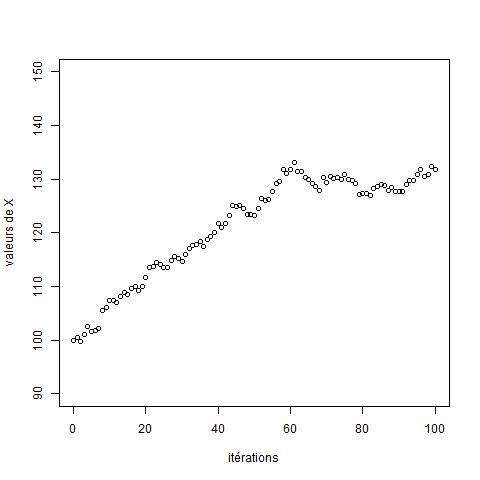
\includegraphics[scale=0.7]{figures/concepts/MC-non-stationnaire.jpeg}
	\caption{
      \label{non-stat}
   Exemple d'une cha\^ine de Markov d'ordre 1 non stationnaire.}
  \end{center}
\end{figure}

%%%%%%%%%%%%%%%%%%%%%
\subsection{Mod\'elisations probabiliste et statistique}\label{confusion.modele}

Les termes de mod\'elisations probabiliste et statistique sont souvent confondus, en particulier dans la litt\'erature d'ing\'enierie.
Cependant, ils poss\`edent des sens diff\'erents. Un mod\`ele probabiliste d\'ecrit par sa densit\'e de probabilit\'e $f_x$ est vou\'e \`a repr\'esenter un  ph\'enom\`ene (ex : physique) r\'eel :
$$
X \sim f_x
$$
tandis que le mod\`ele statistique traduit le fait qu'une ou plusieurs observations de $X$, not\'ee(s) $x^*$, sont reli\'es \`a une r\'ealisation r\'eelle $x$ de $X$ par un dispositif de mesure \index{{bruit de mesure}@{bruit de mesure}} : par exemple
\begin{eqnarray}
x^* & = & x + \epsilon \label{bruit000}
\end{eqnarray}
o\`u $\epsilon$ est un {\it bruit d'observation} dont la nature est al\'eatoire  et qui est souvent suppos\'e gaussien. On notera $f_{\epsilon}$ sa densit\'e, qui est en g\'en\'eral connue\footnote{Notamment {\it via} les sp\'ecifications des constructeurs des dispositifs de mesure, ou par des tests r\'ep\'et\'es dans des conditions contr\^ol\'ees.}. La connaissance de la relation (\ref{bruit000}) permet de d\'efinir la distribution de probabilit\'e de la variable al\'eatoire $X^*$ de r\'ealisation $x^*$ comme une {\it loi de convolution}  de densit\'e $f_{x^*}$
$$
f_{x^*}(u) = \int f_x(u + y) f_{\epsilon}(y) \ dy
$$
et cette loi d\'etermine la {\it vraisemblance statistique} de l'observation $x^*$ (cf. $\S$ \ref{convergence}). 
Toutefois, il est essentiel pour la d\'etermination de $f_x$, enjeu majeur de l'\'etude, que cette loi explique la majeure partie de la variabilit\'e et des valeurs observ\'ees (celles de $X^*$). Souvent, on fera l'hypoth\`ese que l'influence de $\epsilon$ est n\'egligeable, ce qui revient \`a \'ecrire
$$
f_{x^*}(u) \simeq f_x(u) \ \ \ \forall u \in \Omega,
$$
et \`a confondre mod\`eles probabiliste et statistique. Cette hypoth\`ese n'est cependant pas toujours v\'erifi\'ee en pratique, en particulier pour les observations historiques \cite{Reis2005}. Le bruit affectant une mesure peut \^etre important car cette derni\`ere peut :
\begin{itemize}
\item ne pas \^etre directe (par exemple, les mesures de pluie torrentielles ancestrales peuvent \^etre reconstitu\'ees \`a partir d'\'etudes stratigraphiques \cite{Galevski1955}) ;
\item \^etre tr\`es impr\'ecise (exemple : une crue datant du Moyen \^Age a fait l'objet d'une chronique en termes qualitatifs (elle a emport\'e un pont, recouvert des champs...) ou quantitatif avec beaucoup d'incertitude (marque sur un mur de maison d\'emolie depuis) \cite{Coeur2000,Payrastre2003} ;
\item souffrir d'un biais inconnu li\'e \`a un dispositif de mesure mal calibr\'e (ou ab\^im\'e par l'al\'ea lui-m\^eme, surtout s'il est extr\^eme) \cite{FSA-007}.
\end{itemize} 
M\^eme certaines mesures r\'ecentes peuvent souffrir d'un bruit potentiellement fort, car elles sont issues d'un calcul - et non d'une mesure directe - soumis \`a certaines incertitudes (voir \'egalement $\S$ \ref{intro.chapitre.2}). \\



%%%%%%%%%%%%%%%%%%%%%%%%%%%%%%

\subsection{Contr\^ole de l'erreur de mod\'elisation}\label{convergence}

\subsubsection*{Convergence des mod\`eles}\label{conv.modeles}

La fiabilit\'e des mod\`eles probabilistes et statistiques repose sur une approximation du r\'eel dont l'erreur peut \^etre encadr\'ee sous certaines hypoth\`eses techniques. On distingue dans ce cours deux types d'approximation  :
\begin{enumerate}
\item une approximation du comportement inconnu d'une grandeur $X$ consid\'er\'ee comme al\'eatoire (par exemple le maximum d'un \'echantillon sur un intervalle de temps donn\'e) par un comportement th\'eorique (par exemple issu de la th\'eorie statistique des valeurs extr\^emes) permettant de quantifier et d'extrapoler ;
\item une approximation d'un mod\`ele probabiliste th\'eorique par un mod\`ele statistique {\it estim\'e}, au sens o\`u ce mod\`ele th\'eorique implique des param\`etres {\it a priori} inconnus $\theta$, qui seront quantifi\'es grâce aux observations r\'eelles ; puisque ces observations $x_1,\ldots,x_n$ sont consid\'er\'ees comme des r\'ealisations d'une variable al\'etoire $X$, le param\`etre {\it estim\'e} est \'egalement consid\'er\'e comme une r\'ealisation d'une autre variable al\'eatoire $\hat\theta_n$, d\'efinie comme un {\it estimateur statistique}. 
\end{enumerate}
La suite $(\hat\theta_n)_n$ constitue donc un premier processus stochastique, dont on souhaite qu'il approxime  $\theta$ (param\`etre fixe mais inconnu). L'ensemble des variables al\'eatoires $(X_n)_n$ produites alors par le mod\`ele estim\'e forme un deuxi\`eme processus stochastique, dont on souhaite qu'il approxime le comportement r\'eel $X$ (variable al\'eatoire de loi inconnue).   \\
 
Il est donc indispensable de v\'erifier que ces deux types d'approximation n'emp\^echent pas les {\it mod\`eles statistiques estim\'es} - les outils concrets de l'\'etude - de fournir un diagnostic pertinent en termes de reproductibilit\'e des observations, et n'entravent pas significativement leur emploi dans des \'etudes pr\'evisionnelles. Une condition indispensable  est d'avoir {\it convergence} entre mod\'elisation th\'eorique et r\'ealit\'e, puis entre mod\`ele estim\'e et mod\'elisation th\'eorique. Cette convergence s'exprime sous la forme d'un \'ecart entre les protagonistes, qui doit n\'ecessairement diminuer lorsque la quantit\'e d'information (c'est-\`a-dire le nombre d'observations $n$) s'accro\^it jusqu'\`a devenir nul lorsque $n\to\infty$.  \\

Dans le monde probabiliste, cet \'ecart est al\'eatoire, et il est donc possible qu'un \'ecart soit nul sauf en un nombre $k$ de situations donn\'ees,  formant un sous-ensemble de l'espace des \'ev\'enements $\Omega$ de mesure nulle. Typiquement, cet ensemble peut \^etre form\'e d'un nomb\-re fini de valeurs ponctuelles,  ou d'\'el\'ements appartenant \`a la fronti\`ere de $\Omega$ ; en effet, dans le monde continu on sait que (sous des conditions d'ind\'ependance)
\begin{eqnarray*}
\Pm(X\in\{x_1,\ldots,x_m\}) & = & \sum\limits_{i=1}^m \Pm(X=x_i)
\end{eqnarray*}
et que $\Pm(X=x_i)=0$ pour tout $x_i$ (puisque $X$ est continu). On parlera dans ce cas de nullit\'e {\it presque s\^ure}. \index{{consistance}@{consistance}} \index{{convergence presque s\^ure}@{convergence presque s\^ure}} \\

La notion de {\it convergence presque s\^ure} s'en d\'eduit assez naturellement : il s'agit de v\'erifier que la probabilit\'e que la limite d'un processus stochastique $\hat\theta_n$ (ou $X_n$) corresponde \`a la cible $\theta$ (ou $X$) vaut 1 ; ou de fa\c con \'equivalente, que  l'\'ecart entre la limite de ce processus et $\theta$ (ou $X$) est nul presque s\^urement :
\begin{eqnarray*}
X_n \xrightarrow{p.s.} X & \Leftrightarrow & \Pm\left(\lim_{n\to\infty} X_n = X\right) = 1.
\end{eqnarray*}
Cette notion de convergence est la plus forte et la plus courante en pratique pour d\'emontrer le comportement attendu d'un processus al\'eatoire vers une variable al\'eatoire, \'eventuellement r\'eduite \`a un vecteur (ou un scalaire). On parle \'egalement de {\it consistance forte}\footnotemark[1].  \\

\footnotetext[1]{Bien que {\it stricto sensu}, la  {\it consistance} est une propri\'et\'e locale d'un estimateur, qui est induite par la convergence (poss\'edant un sens global).}

D'autres notions de convergence moins fortes, au sens o\`u elles sont entra\^in\'ees par la convergence presque s\^ure, sans r\'eciprocit\'e assur\'ee,  sont \'egalement tr\`es utilis\'ees :
\begin{enumerate}
\item la convergence {\it en probabilit\'e} \index{{convergence en probabilit\'e}@{convergence en probabilit\'e}}
\begin{eqnarray*}
X_n \xrightarrow{{\cal{\Pm}}} X & \Leftrightarrow & \forall \epsilon >0, \ \ \lim\limits_{n\to\infty}\Pm\left(|X_n - X|>\epsilon\right) = 0 
\end{eqnarray*} 
joue un r\^ole important dans un grand nombre de d\'emonstrations de convergences en loi, et implique \'egalement la convergence presque s\^ure d'une sous-suite de $(X_n)_n$ ; elle permet \`a $X_n$ de s'\'ecarter de $X$, mais de moins en moins significativement \`a mesure que $n$ cro\^it ;

\item la convergence {\it en loi}, qui est entra\^in\'ee par la convergence en probabilit\'e et qui constitue l'\'equivalent de la convergence simp\-le\footnote{Au sens de la {\it fonction caract\'eristique} pour les sp\'ecialistes (th\'eor\`eme de continuit\'e de L\'evy \cite{Saporta2006}).} dans le monde probabiliste \index{{convergence en loi}@{convergence en loi}}
\begin{eqnarray*}
X_n \xrightarrow{{\cal{L}}} X & \Leftrightarrow & \lim\limits_{n\to\infty} F_n(x) = F(x)
\end{eqnarray*} 
o\`u $(F_n,F)$ sont les fonctions de r\'epartition de $X_n$ et $X$, respectivement, pour tout $x$ o\`u $F$ est continue. Cette notion de convergence ne caract\'erise pas les valeurs des processus stochastiques, mais uniquement les comportements al\'eatoires : celui de $X_n$ ressemble de plus en plus \`a celui de $X$. On parle alors de {\it consistance faible}\footnotemark[1]. Cette convergence caract\'erise notamment les statistiques de test ($\S$ \ref{test.statistique.classique}).
\end{enumerate}

D'autres notions de convergence (en norme $L^p$ en particulier) sont \'egalement utilis\'ees. Leur emploi est en g\'en\'eral de s'assurer des convergences {\it d\'eterministes} utiles, par exemple celles des esp\'erances (moments), comme l'expriment les deux th\'eor\`emes suivants. \\ 
 
\begin{theorem}
Supposons que $X_n$ converge en norme $L^1$ vers $X$ dans $\Omega\in\R$ :
\begin{eqnarray*}
\lim\limits_{n\to\infty} \E\left[\| X_n - X\|^1\right] & = & 0.
\end{eqnarray*}
Alors $\lim_{n\to\infty}\E[X_n]  =  \E[X]$. \\
\end{theorem}

\begin{theorem}
Supposons que $X_n \xrightarrow{{\cal{L}}} X$ avec $(X_n,X)\in\Omega^2$ avec $\Omega\subset \R$. Alors, pour toute fonction r\'eelle, continue et born\'ee $g$ (en particulier l'identit\'e),
$$
\lim\limits_{n\to\infty}\E[g(X_n)]  =  \E[g(X)]. \\
$$
\end{theorem}

\vspace{0.15cm}

Un ensemble de r\'esultats techniques permet de combiner ces diff\'erentes convergences et leurs transformations par des fonctions continues ({\it mapping theorem}) pour \'etudier des mod\`eles complexes. Pour une exploration approfondie des notions \'evoqu\'ees dans ce paragraphe et leur g\'en\'eralisation dans un monde multidimensionnel, nous sugg\'erons au lecteur l'ouvrage \cite{vandervaart1998}.

%%%%%%%%%%%%%%%%%%%%%%%%%%%%%%%%%%%%%%%%
\subsubsection*{Estimation statistique classique}\label{estimation.stat.classique}

L'{\it inf\'erence} est l'ensemble des m\'ethodologies permettant de cons\-truire un ou plusieurs estimateurs \index{{estimateur statistique}@{estimateur statistique}} de $\theta$ \index{{estimation statistique classique}@{estimation statistique classique}}
$$
\hat{\theta}_n = T(X_1,\ldots,X_n)
$$
o\`u $T$ est une fonction des variables al\'eatoires associ\'ees aux r\'ealisations $x_i$ du ph\'enom\`ene \'etudi\'e. Comme indiqu\'e pr\'ec\'edemment, $\hat\theta_n
$ est donc lui-m\^eme une variable al\'eatoire, et sa valeur {\it observ\'ee} $T(x_1,\ldots,x_n)$ est appel\'ee un {\it estim\'e}. 

\paragraph{Principales propri\'et\'es des estimateurs statistiques}\label{proprietes.estimateur}


Il existe une infinit\'e d'estimateurs possibles pour un vecteur de param\`etre $\theta$, et il est donc indispensable de pouvoir op\'erer une s\'election parmi eux. En statistique classique, %\footnote{o\`u l'on consid\`ere que $\theta$ est fixe et inconnu.}, 
les principales r\`egles utilis\'ees pour classer les estimateurs sont les suivantes :
\begin{enumerate}
\item {\it asymptotiquement} il doit y avoir {\it consistance} :
$$
\hat\theta_n \xrightarrow{?} X
$$
o\`u $?$ repr\'esente, au mieux, la convergence presque s\^ure ;
\item l'{\it erreur quadratique} 
%\footnote{dite aussi en norme $L^2$.} 
\index{{erreur quadratique}@{erreur quadratique}} \index{{moindres carr\'es}@{moindres carr\'es}}
\begin{eqnarray}
\mbox{EQ}(\hat{\theta}_n) = \E\left[(\hat{\theta}_n-\theta)^T (\hat{\theta}_n-\theta)\right], \label{EQ.def}
\end{eqnarray}
doit \^etre la plus faible possible ; celle-ci peut s'\'ecrire comme la somme du d\'eterminant de la matrice de variance-covariance \index{{variance-covariance}@{variance-covariance}} de $\hat{\theta}_n$, qui est une mesure de l'impr\'ecision non-asymptotique de cet estimateur, et du carr\'e du {\it biais}\footnote{Un estimateur $\hat{\theta}_n$ \index{{biais d'un estimateur}@{biais d'un estimateur}} dont l'esp\'erance est \'egale \`a $\theta$ est dit {\it sans biais}.} de l'estimateur 
$$
\mbox{B}(\hat{\theta}_n) = \E\left[\hat{\theta}_n\right] - \theta,
$$
que l'on peut d\'efinir comme l'{\it erreur non-asymptotique} en esp\'erance. Ces deux termes ne peuvent \^etre minimis\'es simultan\'ement, et la minimisation de de (\ref{EQ.def}) proc\`ede donc n\'ecessairement d'un {\it \'equilibre biais-variance}. \index{{\'equilibre biais-variance}@{\'equilibre biais-variance}}. 
%
%aussi appel\'ee {\it biais}, et de l'impr\'ecision non-asymptotique do\^it \^etre le plus faible possible. Ce m\'elange est r\'ealis\'e au travers de l'{\it erreur quadratique} 
%%\footnote{dite aussi en norme $L^2$.} 
%\index{{erreur quadratique}@{erreur quadratique}} \index{{moindres carr\'es}@{moindres carr\'es}}
%$$
%\mbox{EQ}(\hat{\theta}_n) = \E\left[(\hat{\theta}_n-\theta)^T (\hat{\theta}_n-\theta)\right],
%$$
%qui s'\'ecrit \'egalement comme la somme du carr\'e de  $\mbox{B}(\hat{\theta}_n)$ et du    
\end{enumerate}
Remarquons que produire un estimateur $\hat\theta_n$ faiblement consistant  pour un param\`etre inconnu $\theta$ permet de produire un autre estimateur faiblement consistant sur n'importe quelle fonction $h(\theta)$ de ce param\`etre, pourvu que $h$ soit diff\'erentiable. Lorsque la loi de convergence est gaussienne, le proc\'ed\'e de d\'erivation permettant de le cons\-truire est connu sous le nom de {\it m\'ethode Delta}. \\ % et il est d\'etaill\'e au $\S$ \ref{new4.3}.  \\

\begin{theorem}{\bf M\'ethode Delta multivari\'ee}\label{delta.method} \cite{Oehlert1992}. 
Soit $\theta_1,\ldots,\theta_n$ un processus stochastique dans $\R^d$ et soit $g:\R^d\to R^q$ une fonction diff\'erentiable et non nulle en $\theta$. Notons $J_g(\theta)$ la jacobienne de $g$ en $\theta$. Supposons que $\sqrt{n}(\theta_n-\theta)$ converge en loi vers la loi normale multivari\'ee  ${\cal{N}}_d({\bf 0}_d,\Sigma)$, de moyenne le vecteur nul ${\bf 0}_d$ en dimension $d$ et de variance-covariance $\Sigma\in\R^{2d}$. Alors
\begin{eqnarray*}
\sqrt{n}\left(g(\theta_n)-g(\theta)\right) & \xrightarrow{{\cal{L}}} & {\cal{N}}_q\left(0, J^T_g(\theta)\Sigma J_g(\theta)\right).
\end{eqnarray*}
\end{theorem}

\paragraph{Estimation des moindres carr\'es}\label{estimateur.MC}

La classe des {\it estimateurs des moindres carr\'es} (EMC), \index{{moindres carr\'es}@{moindres carr\'es}} qui cherchent \`a r\'ealiser un compromis entre biais et variance, est donc naturellement d\'efinie par une r\`egle du type \index{{compromis biais-variance}@{compromis biais-variance}}
\begin{eqnarray}
\hat{\theta}_n & = & \arg\min_{\hat{\theta}} \widetilde{\mbox{EQ}}(\hat{\theta}) \label{mse.estimateur}
\end{eqnarray}
o\`u $\widetilde{\mbox{EQ}}$ est une approximation empirique de $\mbox{EQ}$, construite comme une fonction de $X_1,\ldots,X_n$. Les estimateurs ainsi produits poss\`edent souvent de bonnes propri\'et\'es de consistance, mais peuvent s'av\'erer sensibles aux choix du mod\`ele et de la param\'etrisation $\theta$. Ainsi, il n'est pas \'evident que l'esp\'erance et/ou la variance impliqu\'ees dans le crit\`ere (\ref{mse.estimateur}) existent. \\

\paragraph{Estimation par maximisation de vraisemblance}\label{estimation.MV}

\paragraph*{Principe de vraisemblance.} \index{{vraisemblance}@{vraisemblance}} \index{{vraisemblance}@{vraisemblance}}
Une r\`egle plus g\'en\'erale est donc n\'ecessairement fond\'ee sur une repr\'esentation plus exhaustive, g\'en\'erique et toujours d\'efinie de l'information apport\'ee par $X_1,\ldots,X_n$ sur le mod\`ele param\'etr\'e par $\theta$. Une telle repr\'esentation est la {\it vraisemblance statistique} $\ell$, qui est d\'efinie (pour des $X_i$ continus) comme la densit\'e jointe des observations $X_i=x_i$ conditionnelle \`a $\theta$. Ainsi,  dans un cas o\`u les observations $x_i$ sont des r\'ealisations iid :
\begin{eqnarray}
\ell(x_1,\ldots,x_n|\theta) & = & \prod\limits_{i=1}^n f_{X}(x_i|\theta). \label{vraisemblance.iid}
\end{eqnarray}  
La vraisemblance peut prendre des formes plus compliqu\'ees lorsque les r\'ealisations ne sont pas ind\'ependantes, non identiquement distribu\'ees %\footnote{partag\'ees entre deux lois diff\'erentes par exemple.}, 
ou sont {\it manquantes} et ont \'et\'e remplac\'ees par des valeurs-seuils, par exemple parce que les limites du proc\'ed\'e de mesure ont \'et\'e atteintes. \\

\begin{exo}\label{censure.vent}{\bf Mesure de la vitesse du vent.} 
\noindent Certains vieux an\'emom\`etres ne peuvent mesurer la vitesse du vent au-del\`a d'une certaine valeur, et remplacent l'observation $x_i$ qui aurait d\^u \^etre faite par une vitesse maximale de vent mesurable, not\'ee $c$. On parle alors d'observation statistique {\it censur\'ee \`a droite}. Ce type d'observation partielle est fr\'equente en {\it analyse de survie} \cite{Mann1974}. Le terme de densit\'e $f(x_i)$ correspondant \`a une observation correcte est alors remplac\'e par la probabilit\'e que la donn\'ee manquante $P(X\geq c)=F(c)$ dans l'\'ecriture de la vraisemblance (\ref{vraisemblance.iid}), o\`u $F$ est la fonction de r\'epartition de $X$. 
\end{exo}

L'exhaustivit\'e de l'information port\'ee par la vraisemblance constitue un principe fondamental de la th\'eorie statistique classique. Alors, l'{\it estimateur du maximum de vraisemblance} \index{{maximum de vraisemblance}@{maximum de vraisemblance}} (EMV)\footnote{Pour des raisons de commodit\'e, on remplace souvent $\ell$ par la log-vraisemblance \index{log-vraisemblance@log-vraisemblance} $\log\ell$ dans la d\'efinition (\ref{mle.intro}).} \index{{maximum de vraisemblance}@{maximum de vraisemblance}} \label{mle.page.ref}
\begin{eqnarray}
\hat{\theta}_n & = & \arg\max \ell(X_1,\ldots,X_n|\theta) \label{mle.intro}
\end{eqnarray}
d\'efinit la variable al\'eatoire dont la r\'ealisation est la {\it valeur la plus probable} de $\theta$ ayant g\'en\'er\'e l'ensemble de r\'ealisations $\{X_i=x_i\}_i$. Par le caract\`ere g\'en\'erique de sa d\'erivation, sa signification et ses bonnes propri\'et\'es de consistance, il est l'estimateur statistique le plus courant et l'un des plus naturels. \\

\begin{exo}\label{censure.intervalle}{\bf Donn\'ees censur\'ees par intervalles.}
\noindent Tr\`es fr\'equemment, une donn\'ee historique unidimensionnelle, ou mal mesur\'ee, peut \^etre simplement d\'ecrite comme une valeur manquante $x_i$ entre deux bornes connues $x_{i,\min}<x_{i,\max}$. Le terme de densit\'e $f(x_i)$ doit alors \^etre remplac\'e dans la vraisemblance (\ref{vraisemblance.iid}) par 
\begin{eqnarray}
P\left(x_{i,\min} \leq X \leq x_{i,\max} | x_{i,\min},x_{i,\max}\right) & & \\
& \hspace{-2cm} = & \hspace{-1cm} P\left(X \leq x_{i,\max} |x_{i,\max}\right) - P\left(X \leq x_{i,\min} |x_{i,\min}\right), \nonumber \\
& \hspace{-2cm} = & \hspace{-1cm} F(x_{i,\max})-F(x_{i,\min}). \label{interval.cens} 
\end{eqnarray}
Si l'on fait de plus l'hypoth\`ese que les valeurs $(x_{i,\min},x_{i,\max})$ sont des donn\'ees elles-m\^emes al\'eatoires (par exemple bruit\'ees), d\'ecrites comme des r\'ealisations de variables $(X_{i,\min},X_{i,\max})$ de lois respectives $f_{i,\min},f_{i,\max})$,  le terme de vraisemblance (\ref{interval.cens}) devient 
\begin{eqnarray*}
\iint P\left(X_{i,\min} \leq X \leq X_{i,\max} | X_{i,\min}=y_1,X_{i,\max}=y_2\right) f_{i,\min}(y_1) f_{i,\max}(y_2) \ dy_1 dy_2.
\end{eqnarray*}
Lorsque la donn\'ee est multivari\'ee, plusieurs situations peuvent se pr\'esenter : une ou plusieurs dimensions de $X$ peuvent \^etre censur\'ees par intervalles, et des traitement approfondis doivent \^etre men\'es pour obtenir des sp\'ecifications statistiques utiles (voir \cite{Kim2002a} pour les analyses de survie, et \cite{sabourin2015semi} pour le cas sp\'ecifique des extr\^emes multivari\'es). \\
\end{exo}

\begin{theorem}{\bf $ \ $ Limite centrale pour l'EMV.}\label{tlc.mle} 
Supposons que $X_1,\ldots,X_n$ soient in\-d\'ependants et identiquement distribu\'es. Soit $q$ la dimension de $\theta$. Alors, sous des conditions de r\'egularit\'e tr\`es g\'en\'erales (dites de Wald),
\begin{eqnarray}
\hat{\theta}_n  & \xrightarrow{{\cal{L}}} & {\cal{N}}_q\left(\theta,I^{-1}_{\theta}\right) \label{LLN.MLE}
\end{eqnarray}
o\`u ${\cal{N}}_q$ repr\'esente la loi normale multivari\'ee en dimension $q$, de variance-covariance $I^{-1}_{\theta}$, et $I_{\theta}$ est la matrice d'information de Fisher \index{Fisher@Fisher} \index{information@information} \index{{information de Fisher}@{information de Fisher}} dont le terme $(i,j)\in\{1,\ldots,q\}^2$ est d\'efini par (sous ces m\^emes conditions de r\'egularit\'e)
\begin{eqnarray}
I^{(i,j)}_{\theta} & = & -\E_X\left[\frac{\partial \log\ell(X_1,\ldots,X_n|\theta)}{\partial \theta_i\partial\theta_j}\right]. \label{info.fisher}\\
\nonumber
\end{eqnarray} 
\end{theorem}

Quelques informations suppl\'ementaires sur la notion d'information et la matrice de Fisher sont indiqu\'ees au $\S$ \ref{info.fisher}. Deux propri\'et\'es importantes de l'EMV sont d'\^etre {\it asymptotiquement sans biais} et {\it fortement consistant et efficace asymptotiquement} : sa covariance asymptotique, fournie par l'inverse de la matrice de Fisher, est {\it minimale} pour tous les estimateurs sans biais de $\theta$. \index{{efficacit\'e asymptotique d'un estimateur}@{efficacit\'e asymptotique d'un estimateur}} 

\paragraph{Information de Fisher}\label{info.fisher}

La notion d'information a \'et\'e propos\'ee dans les ann\'ees 1920 par le chercheur anglais Ronald A. Fisher (consid\'er\'e comme le p\`ere de la statistique math\'ematique). La d\'emarche de Fisher est la suivante: si l'on s'int\'eresse aux caract\'eristiques d'une population nombreuse (voire infinie, qui est le cas limite auquel on est  ramen\'e en permanence), on ne peut ni conna\^itre ni traiter les informations trop abondantes relatives \`a chacun des individus qui la composent. Le probl\`eme devient donc d'\^etre capable de d\'ecrire correctement la population au moyen d'indicateurs de synth\`ese pouvant \^etre fournis par des \'echantillons issus de la population \`a \'etudier. Plus les donn\'ees chiffr\'ees que l'on peut extraire d'un \'echantillon repr\'esentent correctement la population de r\'ef\'erence et plus l'information contenue dans cet \'echantillon doit \^etre consid\'er\'ee comme \'elev\'ee. \\

Partant de cette hypoth\`ese, Fisher a d\'efini techniquement l'information comme la valeur moyenne du carr\'e de la d\'eriv\'ee du logarithme de la loi de probabilit\'e \'etudi\'ee. L'in\'egalit\'e de Cramer permet alors de montrer que la valeur d'une telle information est proportionnelle \`a la faible variabilit\'e -- c'est-\`a-dire au fort degr\'e de certitude -- des conclusions qu'elle permet de tirer. Cette id\'ee, qui est \`a la racine de toute la th\'eorie de l'estimation et de l'inf\'erence statistique, est exactement celle que l'on retrouvera vingt ans plus tard chez Shannon, exprim\'ee cette fois en des termes non plus statistiques mais probabilistes. \\

Si $X$ est un \'echantillon de densit\'e de probabilit\'e $f(x|\theta)$, on d\'efinit l'information de Fisher par 
	\begin{eqnarray*}
	I_{\theta} & = & \E\left[\left(\frac{\partial\log f(X|\theta)}{\partial \theta}\right)^2\right]. 
	\end{eqnarray*}
	Dans le cas o\`u la distribution de probabilit\'e d\'epend de plusieurs param\`etres, $\theta$ n'est plus un scalaire mais un vecteur. %La recherche du maximum de vraisemblance ne se r\'esume donc pas \`a une seule \'equation mais \`a un syst\`eme, et 
	L'information de Fisher n'est plus d\'efinie comme un scalaire mais comme une matrice de covariance appel\'ee matrice d'information de Fisher :
		\begin{eqnarray*}
	I_{\theta_i,\theta_j} & = & \E\left[\left(\frac{\partial\log f(X|\theta)}{\partial \theta_i}\right)\left(\frac{\partial\log f(X|\theta)}{\partial \theta_j}\right)\right] 
	\end{eqnarray*}

\paragraph{Intervalles de confiance}\label{interv.conf}

Dans la pratique, la loi asymptotique de $\hat{\theta}_n$ est \`a son tour estim\'ee en rempla\c cant le terme inconnu $I_{\theta}$ par un estimateur consistant $\hat{I}_n$ (en g\'en\'eral $\hat{I}_n=I_{\hat{\theta}_n}$), ce qui permet de d\'efinir des {\it zones de confiance} $C_{\hat{\theta}_n,\alpha}$ associ\'ees \`a l'estimateur $\hat{\theta}_n$ telles que, lorsque $n$ cro\^it vers l'infini,
\begin{eqnarray}
\Pm\left(\hat{\theta}_n\in C_{\hat{\theta}_n,\alpha}\right) & = & \alpha. \label{confiance.0}
\end{eqnarray}
En particulier, lorsqu'on s'int\'eresse \`a une dimension sp\'ecifique $\theta_i$, le th\'eor\`eme \ref{tlc.mle} permet de d\'efinir l'{\it intervalle de confiance (asymptotique) $1-\alpha$} associ\'e \`a $\hat{\theta}_n$ : 
\begin{eqnarray}
\Pm\left(\theta_i\in\left[\hat{\theta}_{n,i} - z_{\alpha/2}\sqrt{\sigma^2_{i,i}} \ , \ \hat{\theta}_{n,i} + z_{\alpha/2}\sqrt{\sigma^2_{i,i}}\right]\right) & = & 1-\alpha, \label{interv.conf}
\end{eqnarray}
o\`u  $z_{\alpha}$ est le quantile d'ordre $\alpha$ de la loi normale centr\'ee r\'eduite et $\sigma^2_{i,i}$ le terme diagonal $(i,i)$ de l'{\it estim\'e} de l'inverse $\hat{I}^{-1}_n$. \\

 Les \'equations (\ref{confiance.0}) et (\ref{interv.conf}) permettent d'\'evaluer la pr\'ecision de l'estimation de $\theta$ \`a partir de l'\'echantillon $x_1,\ldots,x_n$. Cependant, observons que la mesure de probabilit\'e $\Pm$ dans l'\'equation (\ref{confiance.0}) concerne $\hat\theta_n$ et non $\theta$ (qui est inconnu mais fixe) ; une zone de confiance n'est donc pas d\'efinie par la probabilit\'e $1-\alpha$ que $\theta$ s'y situe, mais comme une zone o\`u il y a {\it a priori} une tr\`es forte probabilit\'e $1-\alpha$ d'obtenir un {\it estim\'e} de $\theta$. En simulant un  grand nombre de fois des \'echantillons similaires \`a $x_1,\ldots,x_n$, la distribution de ces estim\'es a $100(1-\alpha)\%$ chances en moyenne de contenir la vraie valeur $\theta$. L'intervalle de confiance sur une dimension $i$ de $\theta$ vise donc \`a encadrer la vraie valeur $\theta_i$ avec une certaine probabilit\'e reli\'ee \`a la loi asymptotique de l'estimateur $\hat{\theta}_n$, qui pr\'esuppose que le mod\`ele statistique est correct  (et non selon une sorte de probabilit\'e absolue, ind\'ependante de tout mod\`ele). \\  




Tout comme l'EMC, l'EMV n'est pas toujours explicite  et doit \^etre en g\'en\'eral calcul\'e par des m\'ethodes num\'eriques. EMC et EMV peuvent ne pas \^etre uniques pour des mod\`eles complexes, et l'EMV peut aussi ne pas \^etre d\'efini (menant \`a une vraisemblance infinie). Toutefois ces cas restent rares dans le cadre de la th\'eorie des valeurs extr\^emes.  \`A la diff\'erence de l'EMC, l'EMV est toujours invariant par reparam\'etrisation : l'EMV de $h(\theta)$ est $h(\hat{\theta}_n)$ pourvu que $h$ soit une fonction bijective. Cette propri\'et\'e est cruciale pour \'eviter des paradoxes et des inconsistances : si on remplace l'observation $x$ par une transformation bijective $y=d(x)$, le mod\`ele param\'etr\'e par $\theta$ est remplac\'e par un mod\`ele param\'etr\'e par une transformation bijective $\theta'=h(\theta)$. Or l'information apport\'ee par $x$ et $y$ est la m\^eme, et donc toute r\`egle d'estimation $x\to \hat{\theta}(x)$ devrait \^etre telle que $y=d(x)\to \hat{\theta}'(y)=h(\hat{\theta}(x))$. \index{{invariance par reparam\'etrisation}@{invariance par reparam\'etrisation}}\\

Un dernier argument plaide en faveur de l'EMV : la vraisemblance maximis\'ee constitue l'ingr\'edient fondamental de la plupart des techniques de {\it s\'election de mod\`ele} \index{{s\'election de mod\`ele}@{s\'election de mod\`ele}} : assortie d'un facteur de p\'enalisation li\'e au nombre de degr\'es de libert\'e du mod\`ele  \cite{BIC,AIC}, l'{\it estim\'e} de $\ell(x_1,\ldots,x_n|\hat{\theta}_n)$ fournit un diagnostic utile, suppl\'ementaire aux r\'esultats de tests stastistiques, pour \'evaluer la pertinence d'un mod\`ele par rapport \`a un autre sur un m\^eme jeu de donn\'ees. Nous renvoyons le lecteur int\'eress\'e par ce sujet \`a l'ouvrage sp\'ecialis\'e \cite{Planzagl1994}. \\


% %%%%%%%%%%%%%%%%%%%%%%%%%%%%%%%%%%%%%%%%%%%%%%%%%%%%%%
% \subsection{Rappels sur la régression}\label{regression}

% Nous concluons ce rappel en rappelant rapidement les principaux concepts de la {\it r\'egression}  param\'etrique et non param\'etrique, qui s'av\`ereront utiles dans certaines parties des chapitres suivants. Le lecteur int\'eress\'e, et confront\'e \`a la tr\`es vaste litt\'erature consacr\'ee \`a ce sujet, pourra se r\'ef\'erer au r\'ecent ouvrage de Sen et Srivastava \cite{Sen2011}.  L'objectif d'un mod\`ele stochastique de r\'egression  est de d\'eterminer la fa\c con dont l'esp\'erance d'une variable al\'eatoire $Y$ d\'epend des r\'ealisations $x$ d'un vecteur $X\in\chi$ de covariables explicatives, possiblement al\'eatoires \'egalement, au travers de la {\it fonction de r\'egression} (ou de {\it lien}) $g$ :
% \begin{eqnarray*}
% \E[Y|X=x] & = & g(x).
% \end{eqnarray*} 

% \subsubsection{Approche param\'etrique}
              
% \index{{r\'egression param\'etrique}@{r\'egression param\'etrique}}
																																																						
% Une approche param\'etrique consiste \`a injecter dans $f$ une forme {\it a priori} param\'etr\'ee par un nombre fini de param\`etres \`a estimer ; la r\'egression lin\'eaire pr\'esuppose ainsi que
% \begin{eqnarray}
% g(x) & = & \beta_0 + \beta^T x.  \label{reg.lineaire.f}
% \end{eqnarray}
% L'estimation du vecteur $(\beta_0,\beta)$ peut \^etre men\'ee par diff\'erentes approches. Par exemple, la maximisation de vraisemblance est, dans ce cadre, \'equivalente \`a une approche par moindres carr\'es pond\'er\'es, \`a condition de supposer que le mod\`ele complet s'\'ecrit sous la forme
% \begin{eqnarray*}
% Y & = & \beta_0 + \beta^T X + \epsilon
% \end{eqnarray*}
% o\`u $\epsilon$ est un bruit d'esp\'erance nulle, sans corr\'elation, et de variance unique $\sigma^2$, et qu'on dispose d'observations ind\'ependantes de $Y$ et des valeurs de $X$ reli\'ees.

%  En fonction de la dimension de $X$, de $Y$, des hypoth\`eses sur la structure de corr\'elation entre les covariables et/ou entre les dimensions de $Y$,  et enfin en fonction du nombre de donn\'ees disponibles, l'estimation des param\`etres d'un mod\`ele de r\'egression param\'etrique (lin\'eaire ou non) constitue une classe de probl\`emes fondamentaux en statistique. L'objectif fondamental des nombreuses m\'ethodes d'estimation, qui reposent g\'en\'eralement sur une maximisation de la vraisemblance p\'enalis\'ee par un terme de {\it lissage} (ex : r\'egression Lasso, ridge, etc.) est d'assurer un compromis satisfaisant entre pouvoir d'interpolation (biais faible et variance possiblement forte) et  lissage (faible variance mais biais possiblement fort). \\

% \subsubsection{Approche non param\'etrique}\label{reg.non.param}

% \index{{r\'egression non param\'etrique}@{r\'egression non param\'etrique}}

% Une approche non param\'etrique ne postule, {\it a contrario}, aucune forme analytique du type (\ref{reg.lineaire.f}) ni, obligatoirement, un nombre limit\'e de param\`etres d\'efinissant la fonction $g$. Deux grandes familles de m\'ethodes de r\'egression non param\'etriques sont couramment utilis\'ees. Supposons disposer d'un \'echantillon $\{x_i,y_i\}_i$ de r\'ealisations de $(X,Y)$. \\ 

% \begin{enumerate}
% \item La {\bf r\'egression kernel} (ou {\it r\'egression par noyau}) \cite{Nadaraya1964,Watson1964} proposent d'estimer $g$ par un estimateur \`a noyau d\'efini par
% \index{{r\'egression kernel}@{r\'egression kernel}}
% \begin{eqnarray*}
% \hat{g}_h(x) & = & \sum\limits_{i=1}^n \omega_i(x,h) y_i
% \end{eqnarray*}
% avec
% \begin{eqnarray*}
% \omega_i(x,h) & = & \frac{K\left(\frac{x_i-x}{h}\right)}{\sum\limits_{j=1}^n K\left(\frac{x_j-x}{h}\right)}
% \end{eqnarray*}
% o\`u $K(u)=K((x-i-x)/h)$ d\'efinit une fonction noyau ({\it kernel}) -- c'est-\`a-dire une densit\'e de probabilit\'e maximale en 0 et uniquement fonction de la distance $|x_i-x|$ (donc sym\'etrique) -- et $h$ un param\`etre de lissage (nomm\'e {\it largeur de bande}, ou {\it bandwidth}). On note que chaque poids $\omega_i(x,h)$ d\'ecro\^it en fonction de la distance $|x_i-x|$, et cro\^it \`a mesure que $h$ est \'elev\'e. La s\'election de $h$ r\'esulte \`a la fois d'un compromis biais-variance et d'un arbitrage sur la r\'egularit\'e de la courbe $x\mapsto \hat{g}_h(x)$ (lisse versus irr\'eguli\`ere), qui est tr\`es g\'en\'eralement produit par minimisation approch\'ee d'un crit\`ere $C(h)$ d\'efini comme l'erreur quadratique moyenne int\'egr\'ee ({\it Mean Integrated Squared Error}, ou MISE) 
% \begin{eqnarray*}
% C(h) & = & \E\left[\int_{\chi}\left( \hat{g}(x,h) - g(x)\right)^2 \ dx\right]; 
% \end{eqnarray*}   
% \index{{MISE}@{MISE}}
% ce crit\`ere n'\'etant pas utilisable ($g$ \'etant inconnue), il est typiquement remplac\'e par un crit\`ere de validation crois\'ee entre les $y_i$ et chaque pr\'edicteur $\hat{g}_{-i}(x_i,h)$ produit par l'utilisation de l'ensemble de l'\'echantillon except\'e le point $(x_i,y_i)$.  \\


% \item La {\bf r\'egression locale polynomiale} constitue une alternative \`a l'approche pr\'ec\'edente, qui se r\'ev\`ele plus robuste aux valeurs extr\^emes de $X$ en termes d'estimation de $g$. Elle postule que la fonction $g(x)$ \'evalu\'ee au point $x$ peut \^etre approxim\'ee par la valeur d'une fonction param\'etrique estim\'ee dans un voisinage ({\it localement}) ${\cal{V}}(x)$ de ce point $x$. Il est par exemple envisageable d'approximer $g(x)$ par un polyn\^ome de degr\'e 1
% \index{{r\'egression locale polynomiale}@{r\'egression locale polynomiale}}
% \begin{eqnarray*}
% \hat{g}(x) & = & \hat{\alpha}(x) + \hat{\beta}(x)^T x
% \end{eqnarray*}
% o\`u les estimateurs $\hat{\alpha}(x)$ et $\hat{\beta}(x)$ sont d\'etermin\'es par la minimisation du crit\`ere pond\'er\'e
% \begin{eqnarray*}
% \sum\limits_{x_i\in{\cal{V}}(x)} \omega'_i\left(y_i - \hat{\alpha}(x) + \hat{\beta}(x)^T x_i\right)^2.
% \end{eqnarray*}
%  o\`u le poids $\omega'_i$ peut \^etre constant (r\'egression LOESS \cite{Cleveland_1979}) ou \^etre l\`a encore d\'efini {\it via} l'emploi d'une fonction kernel (r\'egression LOWESS \cite{Cleveland_1988}). \\

% \index{{r\'egression LOESS}@{r\'egression LOESS}}
% \index{{r\'egression LOWESS}@{r\'egression LOWESS}}
	
% \end{enumerate}




